% -*- latex -*-
%%%%%%%%%%%%%%%%%%%%%%%%%%%%%%%%%%%%%%%%%%%%%%%%%%%%%%%%%%%%%%%%
%%%%
%%%% This TeX file is part of the tutorial
%%%% `Introduction to the PETSc library'
%%%% by Victor Eijkhout, eijkhout@tacc.utexas.edu
%%%%
%%%% copyright Victor Eijkhout 2012-2022
%%%%
%%%%%%%%%%%%%%%%%%%%%%%%%%%%%%%%%%%%%%%%%%%%%%%%%%%%%%%%%%%%%%%%

\lstset{language=C}
\sectionframe{\texttt{Vec} datatype: vectors}

%\subsection{Basic stuff}

\begin{details}
\begin{numberedframe}{Create calls}
\small
Everything in PETSc is an object, with create and destroy calls:
\begin{lstlisting}
VecCreate(MPI_Comm comm,Vec *v);
VecDestroy(Vec *v);

/* C */
Vec V;
VecCreate(MPI_COMM_WORLD,&V);
VecDestroy(&V);
\end{lstlisting}
\end{numberedframe}

\lstset{language=Fortran}
\begin{fortran}
\begin{numberedframe}{Create calls, Fortran}
\begin{lstlisting}
! Fortran
Vec V
call VecCreate(MPI_COMM_WORLD,V,e)
call VecDestroy(V,e)
\end{lstlisting}
Note: in Fortran there are no `star' arguments
\end{numberedframe}
\end{fortran}
\lstset{language=C}

\begin{numberedframe}{More about vectors}
A vector is a vector of \lstinline{PetscScalar}s: there are no vectors of
integers (see the \lstinline{IS} datatype later)

The vector object is not completely created in one call:
\begin{lstlisting}
VecSetType(V,VECMPI) // or VECSEQ
VecSetSizes(Vec v, int m, int M);
\end{lstlisting}
Other ways of creating: make more vectors like this one:
\begin{lstlisting}
VecDuplicate(Vec v,Vec *w);
\end{lstlisting}
\end{numberedframe}

\end{details}

\lstset{language=Python}  
\begin{python}
\begin{numberedframe}{Python}
  Create is a class method:

  \pverbatimsnippet{pyveccreate}
\end{numberedframe}
\end{python}
\lstset{language=C}

\begin{numberedframe}{Parallel layout up to PETSc}
\begin{lstlisting}
VecSetSizes(Vec v, int m, int M);
\end{lstlisting}
Local size can be specified as \lstinline{PETSC_DECIDE}.

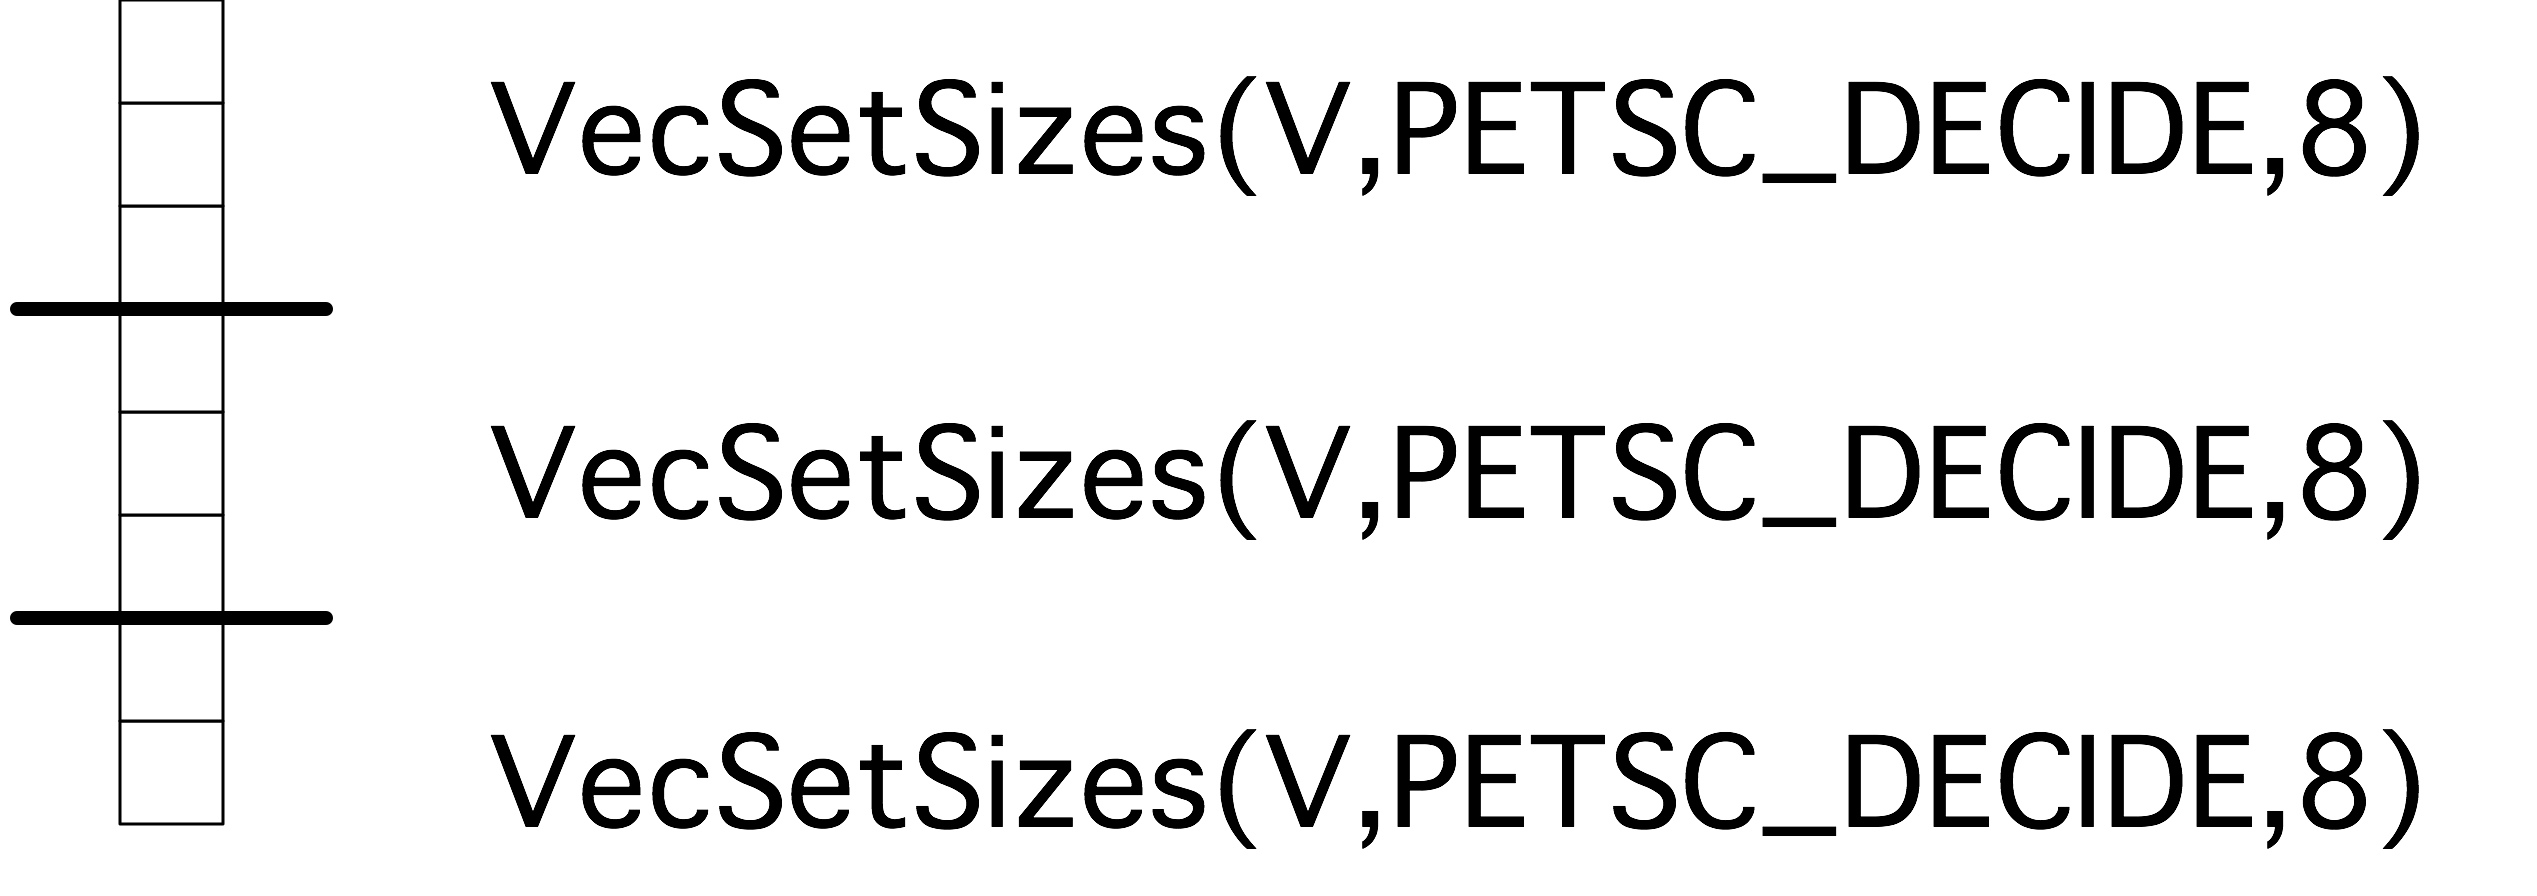
\includegraphics[scale=.08]{veccreate2}
\end{numberedframe}

\begin{numberedframe}{Parallel layout specified}
Local or global size in
\begin{lstlisting}
VecSetSizes(Vec v, int m, int M);
\end{lstlisting}
Global size can be specified as \lstinline{PETSC_DECIDE}.

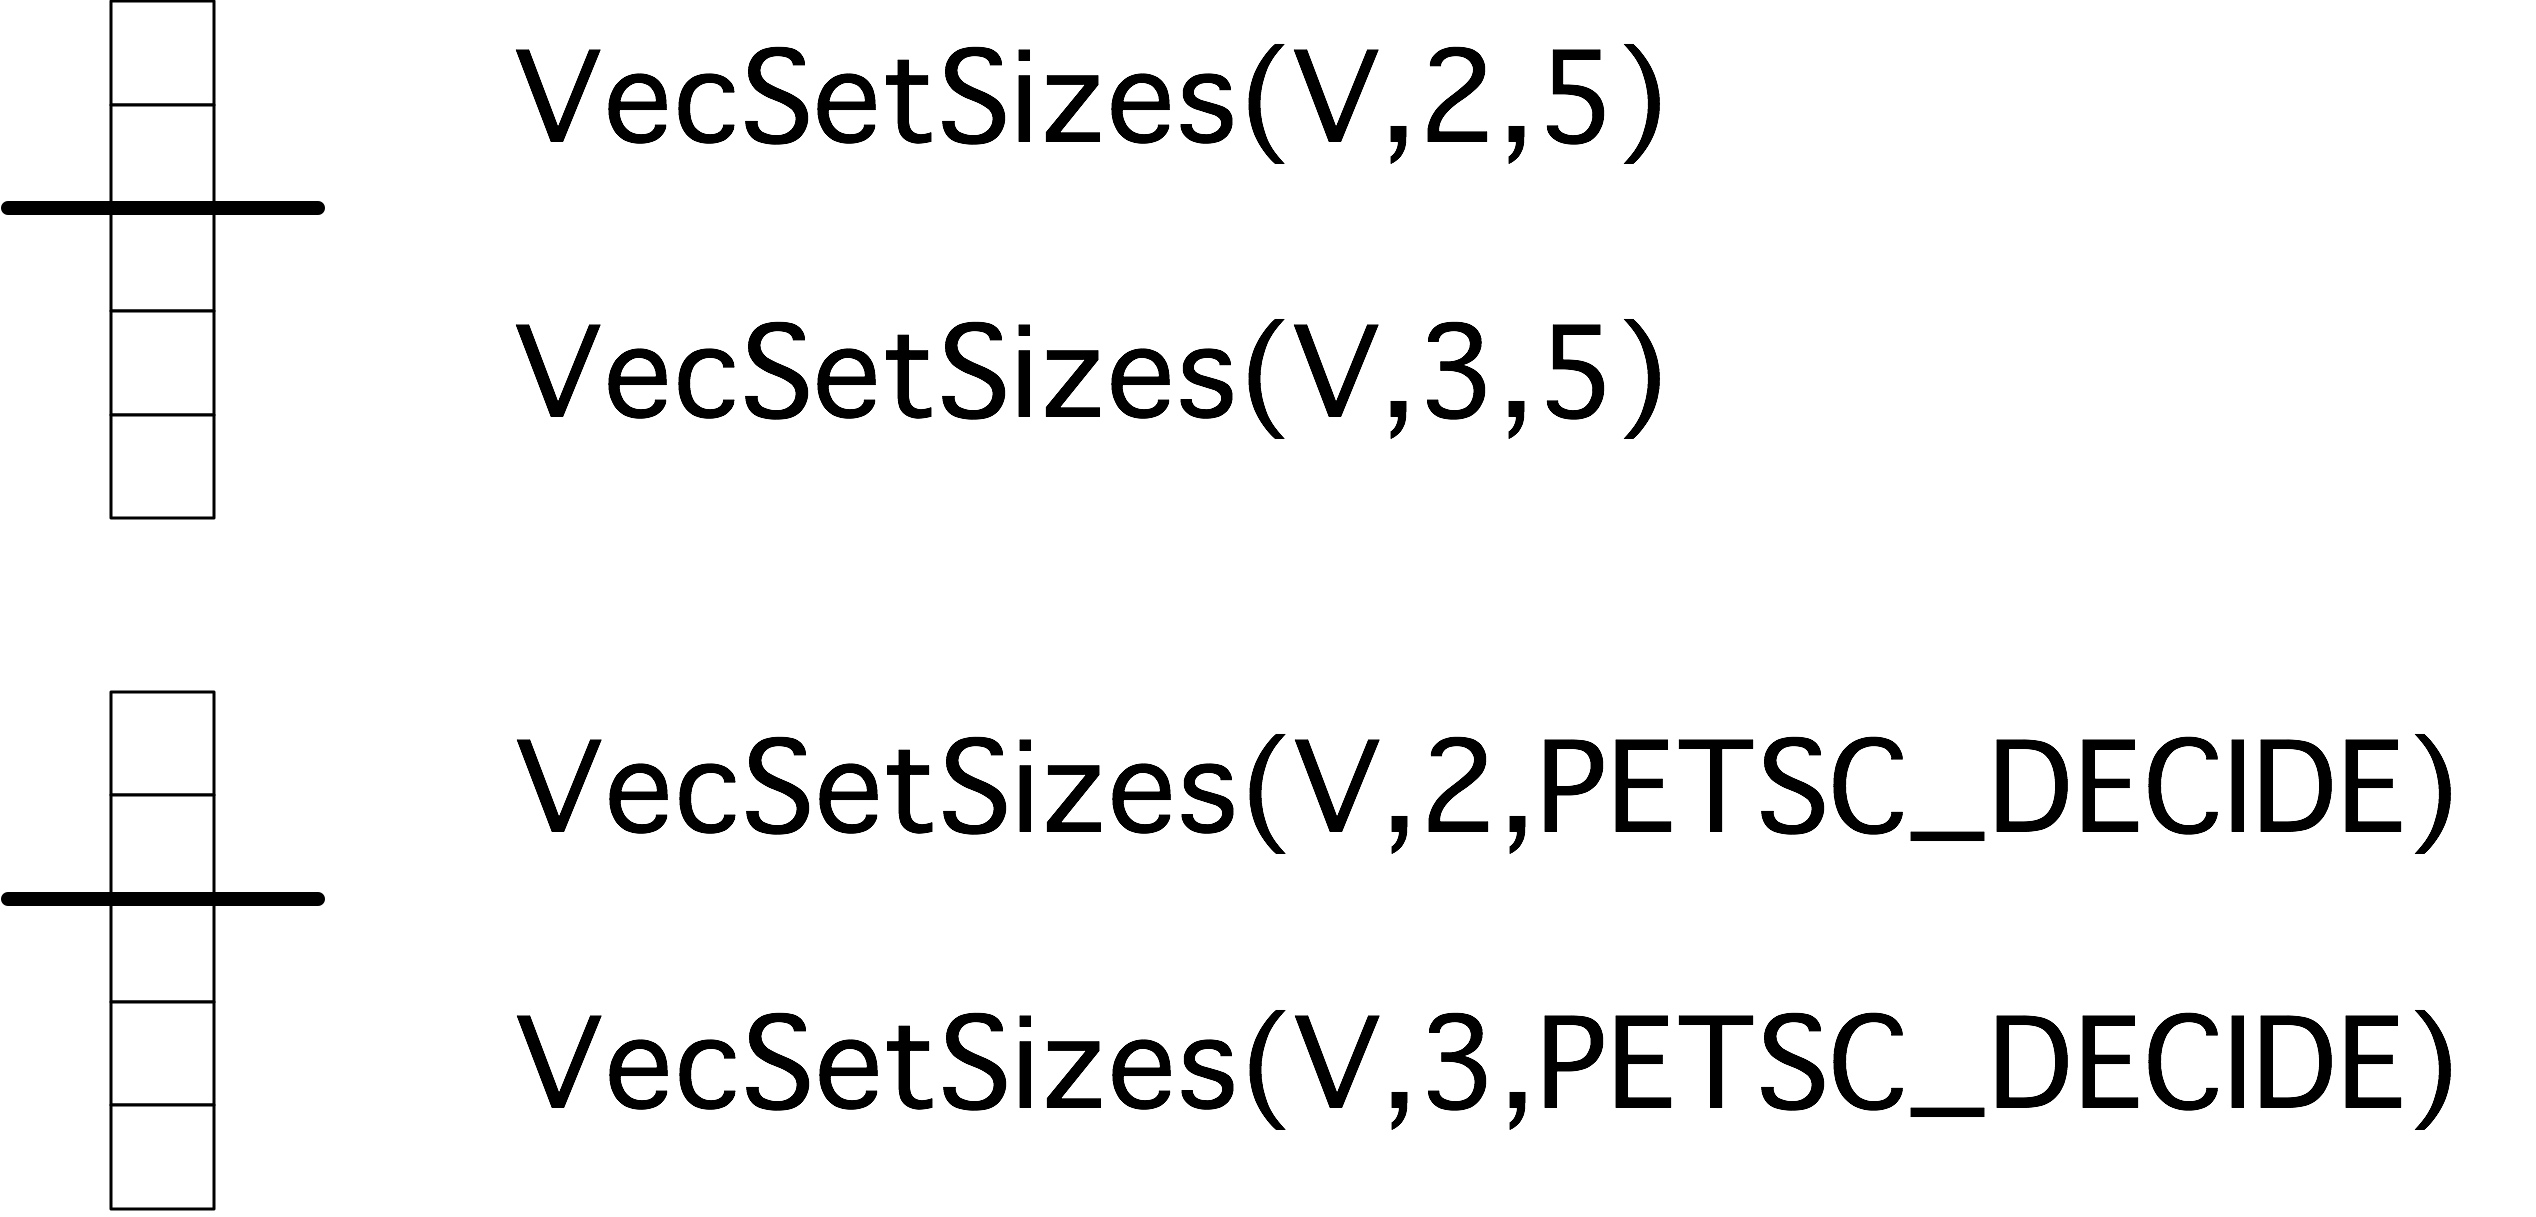
\includegraphics[scale=.08]{veccreate1}
\end{numberedframe}

\lstset{language=Python}
\begin{python}
\begin{numberedframe}{Vector layout in python}
  Local and global sizes in a tuple,\\
  \plstinline{PETSc.DECIDE} for parameter not specified.
  
  \pverbatimsnippet{pyvecsize}
\end{numberedframe}
\end{python}
\lstset{language=C}

\begin{details}
  %%%%
  %%%% ownership querying
  %%%%
\begin{numberedframe}{Query parallel layout}
Query vector layout:
\begin{lstlisting}
VecGetSize(Vec,PetscInt *globalsize)
VecGetLocalSize(Vec,PetscInt *localsize)
VecGetOwnershipRange(Vec x,PetscInt *low,PetscInt *high)
\end{lstlisting}
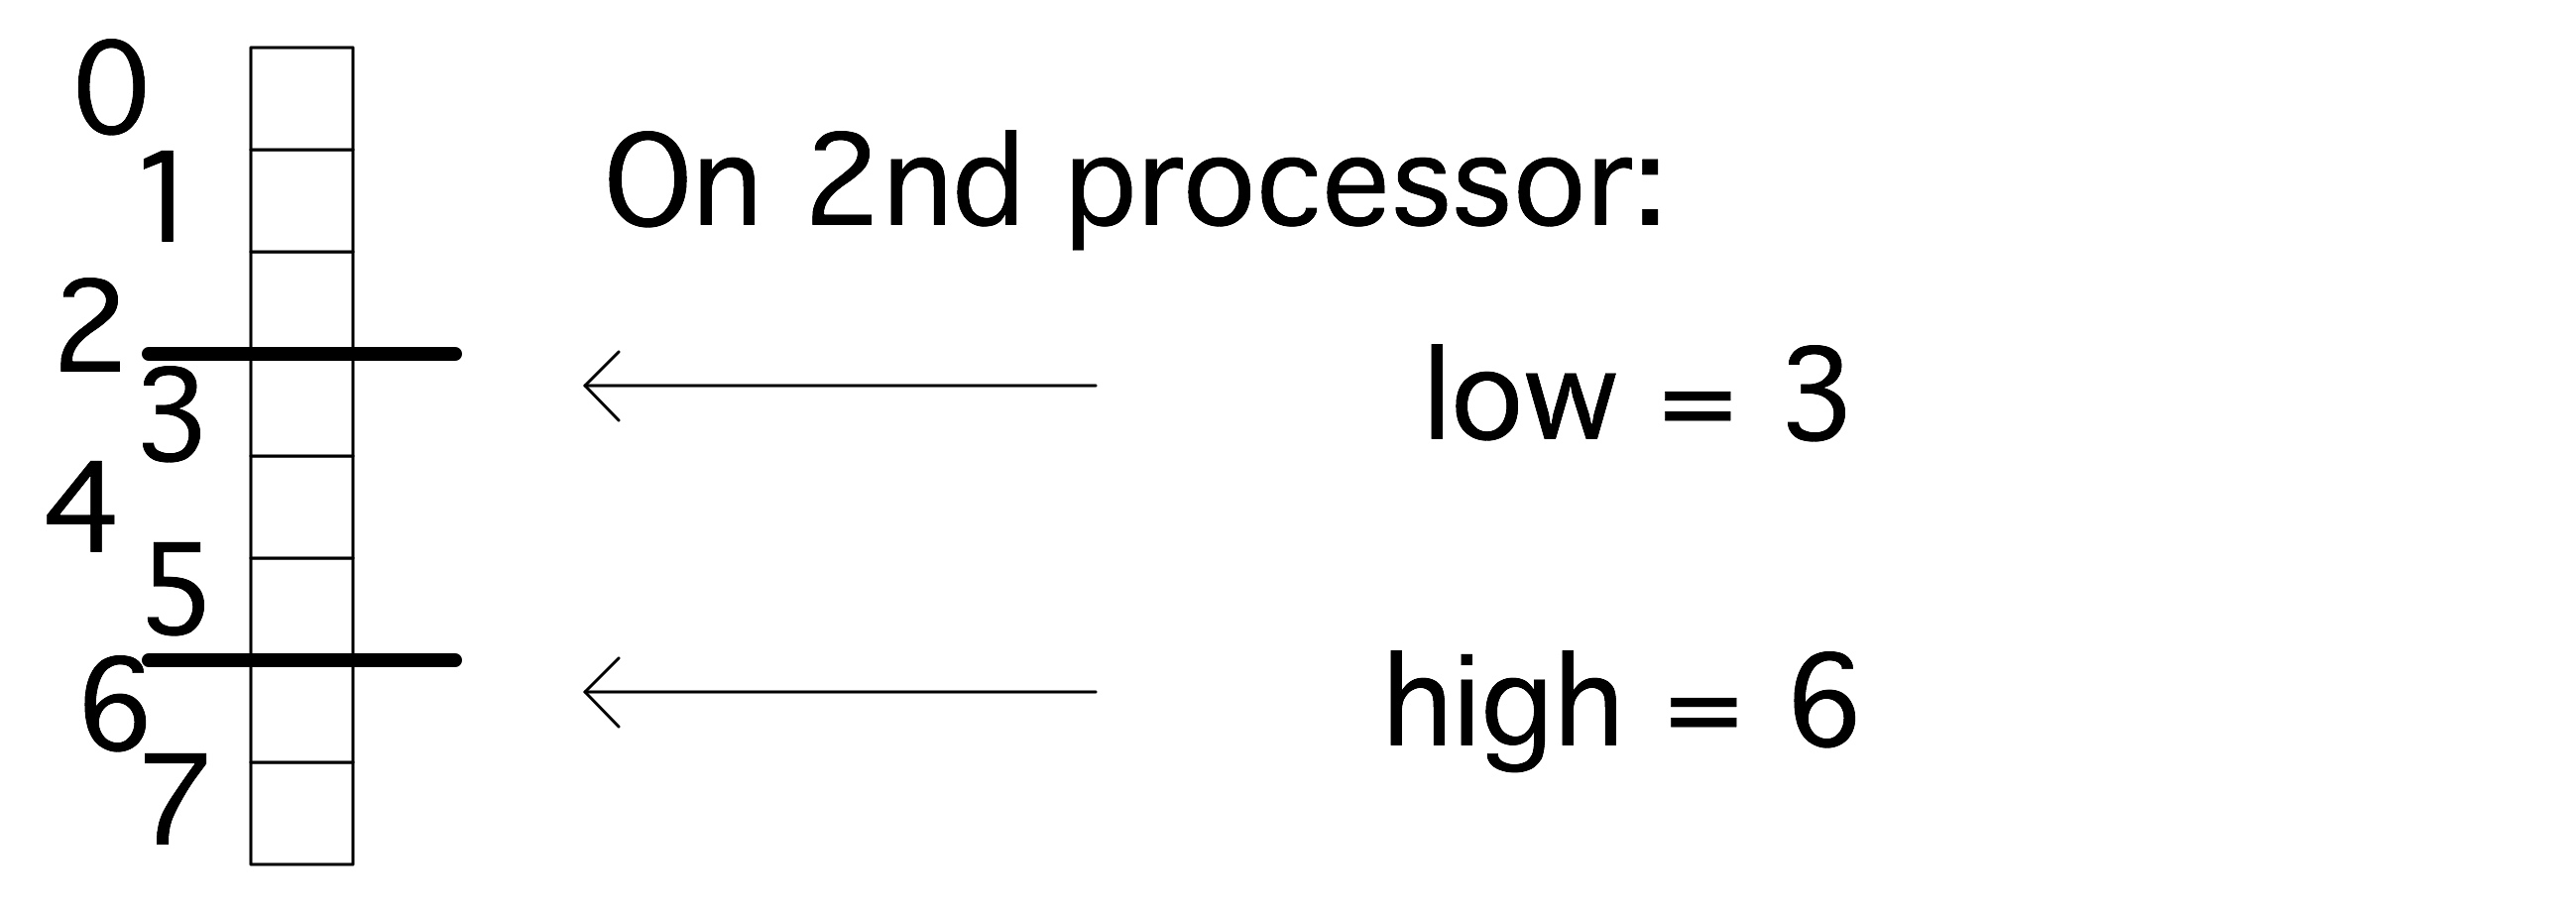
\includegraphics[scale=.08]{veclayout}
\end{numberedframe}

\begin{numberedframe}{Layout, regardless object}
Query general layout:
\begin{lstlisting}
PetscSplitOwnership(MPI_Comm comm,PetscInt *n,PetscInt *N);
\end{lstlisting}
(get local/global given the other)
\end{numberedframe}
\end{details}

\begin{numberedframe}{Setting values}
\small
Set vector to constant value:
\begin{lstlisting}
VecSet(Vec x,PetscScalar value);
\end{lstlisting}
Set individual elements (global indexing!):
\lstset{language=Fortran}
\begin{lstlisting}
VecSetValue
   (Vec x,int row,PetscScalar value,
    InsertMode mode);

i = 1; v = 3.14;
VecSetValue(x,i,v,INSERT_VALUES);

call VecSetValue(x,i,v,INSERT_VALUES)
\end{lstlisting}
The other insertmode is \indexpetscshow{ADD_VALUES}.
\end{numberedframe}

\lstset{language=C}

\begin{numberedframe}{Setting values by block}
Set individual elements (global indexing!):
\begin{lstlisting}
VecSetValues(Vec x,int n,int *rows,PetscScalar *values,
    InsertMode mode); // INSERT_VALUES or ADD_VALUES

ii[0] = 1; ii[1] = 2; vv[0] = 2.7; vv[1] = 3.1;
VecSetValues(x,2,ii,vv,INSERT_VALUES);

ii(1) = 1; ii(2) = 2; vv(1) = 2.7; vv(2) = 3.1
call VecSetValues(x,2,ii,vv,INSERT_VALUES,ierr,e)
\end{lstlisting}
\end{numberedframe}

\begin{python}
\begin{numberedframe}{Setting values: Python}
  \pverbatimsnippet{pyvecval}
  \pverbatimsnippet{pyvecvals}
\end{numberedframe}
\end{python}

\begin{numberedframe}{Setting values}
No restrictions on parallelism;\\
after setting, move values to appropriate processor:
\begin{lstlisting}
VecAssemblyBegin(Vec x);
VecAssemblyEnd(Vec x);
\end{lstlisting}
`Latency hiding':\\
some of the implementation is visible here
to the user
\end{numberedframe}

\begin{numberedframe}{Basic operations}
\small
\begin{lstlisting}
VecAXPY(Vec y,PetscScalar a,Vec x);   /* y <- y + a x */
VecAYPX(Vec y,PetscScalar a,Vec x);   /* y <- a y + x */
VecScale(Vec x, PetscScalar a);
VecDot(Vec x, Vec y, PetscScalar *r); /* several variants */
VecMDot(Vec x,int n,Vec y[],PetscScalar *r);
VecNorm(Vec x,NormType type, PetscReal *r);
VecSum(Vec x, PetscScalar *r);
VecCopy(Vec x, Vec y);
VecSwap(Vec x, Vec y);
VecPointwiseMult(Vec w,Vec x,Vec y);
VecPointwiseDivide(Vec w,Vec x,Vec y);
VecMAXPY(Vec y,int n, PetscScalar *a, Vec x[]);
VecMax(Vec x, int *idx, double *r);
VecMin(Vec x, int *idx, double *r);
VecAbs(Vec x);
VecReciprocal(Vec x);
VecShift(Vec x,PetscScalar s);
\end{lstlisting}
\end{numberedframe}

\begin{exerciseframe}[vec]
  Create a vector where the values are a single sine wave.
  using \indexpetscshow{VecGetSize}, \indexpetscshow{VecGetLocalSize},
  \indexpetscshow{VecGetOwnershipRange}.
  Quick visual inspection:
\begin{verbatim}
ibrun vec -n 12 -vec_view
\end{verbatim}
\end{exerciseframe}

\begin{exerciseframe}[vec]
Use the routines \lstinline{VecDot}, \lstinline{VecScale} and \lstinline{VecNorm} to
compute the inner product of vectors \lstinline{x,y}, scale the vector~\lstinline{x},
and check its norm:
\[
\begin{array}{l}
p \leftarrow x^ty\\
x \leftarrow x/p\\
n \leftarrow \|x\|_2\\
\end{array}
\]
\end{exerciseframe}

\begin{details}
\begin{numberedframe}{Split dot products and norms}
  MPI is capable (in principle) of `overlapping computation and communication'.
  \begin{itemize}
  \item Start inner product~/ norm with \indexpetscshow{VecDotBegin}~/
    \indexpetscshow{VecNormBegin};
  \item Conclude inner product~/ norm with \indexpetscshow{VecDotEnd}~/
    \indexpetscshow{VecNormEnd};
  \end{itemize}
  Also: start/end multiple norn/dotproduct operations.
\end{numberedframe}
\end{details}

\begin{details}
\begin{numberedframe}{Direct access to vector values (C)}
 Setting values is done without user access to the stored data\\
 Getting values is often not necessary: many operations provided.\\
 what if you do want access to the data?

 Solution~1. Create vector from user provided array:
\begin{lstlisting}
VecCreateSeqWithArray(MPI_Comm comm,
  PetscInt n,const PetscScalar array[],Vec *V)
VecCreateMPIWithArray(MPI_Comm comm,
  PetscInt n,PetscInt N,const PetscScalar array[],Vec *vv)
\end{lstlisting}
\end{numberedframe}

\begin{numberedframe}{Direct access'}
  Solution~2.
  Retrive the internal array:
\begin{lstlisting}
VecGetArray(Vec x,PetscScalar *a[])
/* do something with the array */
VecRestoreArray(Vec x,PetscScalar *a[])
\end{lstlisting}
Note: local only; see \lstinline{VecScatter} for more general
mechanism)
\end{numberedframe}

\begin{numberedframe}{Getting values example}
\begin{lstlisting}
int localsize,first,i;
PetscScalar *a;
VecGetLocalSize(x,&localsize);
VecGetOwnershipRange(x,&first,PETSC_NULL);
VecGetArray(x,&a);
for (i=0; i<localsize; i++)
  printf("Vector element %d : %e\n",first+i,a[i]);
VecRestoreArray(x,&a);
\end{lstlisting}
Fortran: \lstinline{PETSC_NULL_INTEGER}
\end{numberedframe}

\begin{numberedframe}{More array juggling}
  \begin{itemize}
  \item
    \indexpetscshow{VecPlaceArray}: replace the internal array;
    the original can be restored with \indexpetscshow{VecRestoreArray}
  \item \indexpetscshow{VecReplaceArray}: replace and free the internal array.
  \end{itemize}
\end{numberedframe}

\lstset{language=Fortran}
\begin{fortran}
\begin{numberedframe}{Array handling in F90}
\begin{lstlisting}
    PetscScalar, pointer :: xx_v(:)
    ....
    call VecGetArrayF90(x,xx_v,ierr)
    a = xx_v(3)
    call VecRestoreArrayF90(x,xx_v,ierr)
\end{lstlisting}
More seperate F90 versions for `Get' routines\\
(there are some ugly hacks for F77)
\end{numberedframe}
\end{fortran}

\end{details}
\lstset{language=C}

